\chapter{Validation of Application Energy Monitoring}
\label{chapter:validation}

\section{Introduction}

As described in \cref{chapter:implementation} we have implemented a proof-of-concept version of the Apollo Energy Allocator system, to prove the usefulness of our approach for allocating energy of underlying host systems to individual application requests running on them.  The software was tested during development to ensure correctness with respect to expected results through unit and integration tests, but now needs to be validated by using it in realistic test cases.  This process is described in this chapter.

In order to validate Apollo with realistic test cases, we need to define the kind of validation we are interested in achieving.  There are two main varieties of validation that we wish to achieve.

Firstly we wish to validate the \emph{consistency} of Apollo's results across a range of scenarios, to ensure that energy is allocated consistently with respect to the workload in the execution scenarios and host utilisation levels that prevail during them.

Next, we need to validate the \emph{allocation} of Apollo's results when a specific application scenario is run on a host machine with different amounts of competing workload.  As the competing workload rises, the energy allocation to the application scenario should fall, in proportion to its use of the machine.

We also wish to validate the \emph{calculation correctness} of Apollo's results, by running the calculator in one or more controlled scenarios where we can also gather additional runtime statistics that allow a separate independent calculation of a fair energy consumption and manually perform these calculations and use them to check the correctness of Apollo's results in the same scenarios.

Finally, an additional area of validation we wish to perform is to confirm that \emph{CPU is a valid proxy for overall resource usage} when performing energy allocation calculations.  For this validation we focus on how CPU usage varies for disk IO intensive workloads.

\section{Testing Approach}

\subsection{The Test Application}
TODO - explain the microservice app

\subsection{The Test Software}
TODO - explain how tests were run and results captured

\section{Validating Consistency}

To validate consistency of energy allocation, our strategy is to run a known control workload under fixed host utilisation conditions (no other workload being the simplest case) and to run a range of other workloads that we know contain an equivalent amount of computational work but are structured differently.  The energy allocation should be the same for each case.

In our first test, we structured a workload into three cases, each of which involved the same amount of CPU workload but in three different scenarios.  The first scenario invoked a short service call (involving 50msec of CPU work) 1000 times, the second scenario invoked a longer service call (500msec of CPU work) 100 times and the third ran a long service call (5000msec of CPU work) 10 times.  Each scenario was called 6 times to ensure a consistent result.

Our first question was whether the energy allocations per request were consistent across the three cases.  Our analysis of this question is shown in the scatter graph in \fref{figure:validation-energycpu}, which plots the energy usage against CPU workload for each of the scenarios executed, using logarithmic scales.

\begin{figure}
\centering
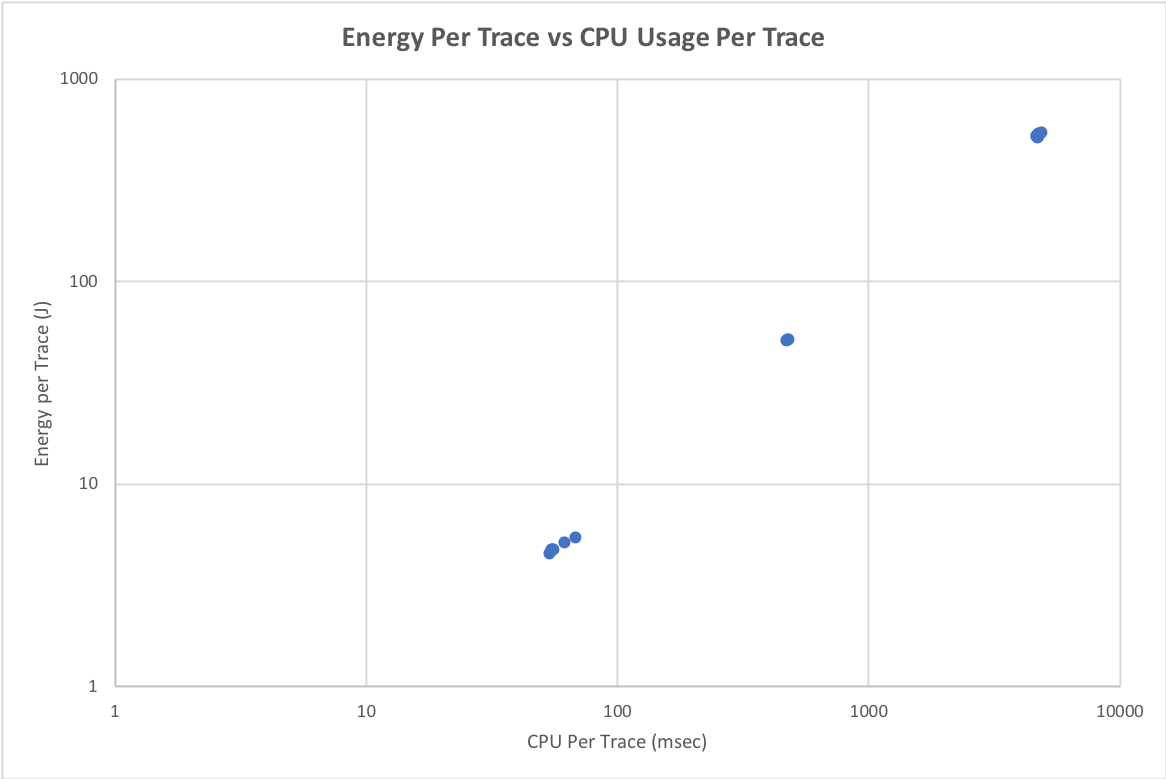
\includegraphics[width=1.0\textwidth]{Figures/validation-energycpu}
\caption{Energy Allocation per Request for Small, Medium and Large Services}
\label{figure:validation-energycpu}
\end{figure}

The graph shows the three sets of scenarios (short, medium and long) clearly clustering very closely, showing that the energy allocation per trace is extremely consistent across the three sets, suggesting that the allocation calculation is working consistently as designed.  More precisely, the correlation coeficient between the two sets of values is 0.999, indicating a very high degree of correlation between CPU consumed and energy allocation performed.

We also wanted to understand how consistent the energy allocation per trace was across the three service request sets and to do this we calculated the CPU to energy ratio as $CPU msec / Energy J$ for each of the results we had from this test set.  The results of this calculation are presented in \tref{table:energypermsec}.

\begin{table}
\centering
\caption{Energy Allocation per Millisecond}
\label{table:energypermsec}
\footnotesize
\begin{tabular}{|l|r|r|}
\hline
\textbf{Request Length} & \textbf{Average J/msec}  & \textbf{Stddev J/msec} \\
\hline
50 msec & 0.0848 & 0.0026 \\
\hline
500 msec & 0.1094 & 0.0005 \\
\hline
5000 msec & 0.1121 & 0.0017 \\
\hline
\end{tabular}
\end{table} 

As can be seen, the energy allocation per CPU millisecond is slightly different between the three cases, with a consistent trend to increase slightly as the number of milliseconds of CPU time per request increases by an order of magnitude each time.  As can also be seen the standard deviation values are very small, indicating that the averages are representative of the data.

When we analysed these values a little we noticed that the difference between the average for the 50 msec case and the 500 msec case was 0.0246, while the difference between the 500 msec case and the 5000 msec case was 0.0027.  So the difference in mean values differs by the same order of magnitude as the length of the workload in each case.  The length of the workload is inversely proportional to the number of service requests made, therefore we think the lower energy per millisecond for the short requests indicates the lower intensity of workload that the scenario places the server under.  As much of the time in this scenario will be waiting for network operations to receive or transmit data from and to the client, the intensity of the CPU operation will be lower and so the allocation algorithm results in a (slightly) lower amount of energy per CPU millisecond of work.






\section{Validating Allocation}

\section{Validating Calculation}

\section{Validating CPU as a Resource Usage Proxy}

\section{Summary}

